\documentclass[11pt]{article}
\usepackage[utf8]{inputenc}
\usepackage[T1]{fontenc}
\usepackage{amsmath,amssymb}
\usepackage{graphicx}
\usepackage{booktabs}
\usepackage{hyperref}
\usepackage{xcolor}
\usepackage{multirow}
\usepackage[margin=1in]{geometry}
\usepackage{natbib}
\usepackage{caption}
\usepackage{subcaption}
\usepackage{enumitem}

\title{Does Experience Make LLMs Faster? Temporal Pattern Augmentation Across Six Foundation Models}
\author{Anand Karasi\\Independent Researcher\\\texttt{karasi@alum.mit.edu}}
\date{February 2026}

\begin{document}
\maketitle

\begin{abstract}
We investigate whether augmenting large language model (LLM) prompts with historical problem-solving patterns---temporal pattern augmentation---improves performance on code debugging tasks. Testing six foundation models from three providers (Claude Opus 4.5/4.6, GPT-5.2/5.2 Pro, Gemini 2.5 Flash/3.0 Pro) on 28 debugging tasks via direct API calls, we find that temporal augmentation provides \textbf{no benefit for five of six models} and produces a modest speedup (\textbf{+10.8\%}) only for Gemini 2.5 Flash, the least capable model tested. Stronger models show slight degradation ($-1.2\%$ to $-5.1\%$). These results contradict an earlier finding of 47\% speedup, which we trace to a measurement artifact in orchestration-layer benchmarking. Our findings suggest that state-of-the-art LLMs already internalize the patterns that temporal augmentation provides, and that additional context may introduce processing overhead without corresponding benefit. We discuss implications for the ``more context is better'' assumption prevalent in LLM augmentation research and provide practical guidelines for when pattern augmentation may or may not help.

\medskip
\noindent\textbf{Code and data:} \url{https://github.com/engagedirect001/temporalintelligence}
\end{abstract}

%% ═══════════════════════════════════════════════════════════════
\section{Introduction}
\label{sec:intro}

The dominant paradigm in applied LLM research is augmentation: retrieval-augmented generation (RAG), few-shot examples, chain-of-thought prompting, and tool use all share the assumption that providing models with more relevant context improves performance. This assumption is well-supported for many tasks, particularly when models lack domain-specific knowledge \citep{lewis2020retrieval, brown2020language}.

But does augmentation always help? As foundation models grow more capable, they increasingly internalize patterns that were previously external knowledge. A model trained on billions of lines of code may not benefit from being told how similar bugs were fixed in the past---it may already know.

We test this hypothesis through \emph{temporal pattern augmentation}: injecting structured historical problem-solving patterns (prior bug descriptions, solution strategies, and timing metadata) into LLM prompts for code debugging tasks. We compare a \textsc{Stateless} condition (task only) against a \textsc{Temporal} condition (task plus historical patterns) across six models spanning three capability tiers.

Our results are a negative finding that we believe is important:
\begin{itemize}[nosep]
    \item Five of six models show no benefit or slight degradation from temporal augmentation.
    \item Only Gemini 2.5 Flash, the least capable model tested, shows improvement (+10.8\%).
    \item An earlier reported 47\% speedup was an artifact of orchestration-layer measurement, not genuine model acceleration.
\end{itemize}

These findings have practical implications: practitioners should not assume that injecting historical patterns into prompts will improve performance for capable models, and the benchmarking community should be vigilant about measurement artifacts when evaluating LLM augmentation strategies.

%% ═══════════════════════════════════════════════════════════════
\section{Related Work}
\label{sec:related}

\paragraph{Retrieval-Augmented Generation.} RAG systems augment LLM prompts with retrieved documents to provide factual grounding \citep{lewis2020retrieval}. While effective for knowledge-intensive tasks, the marginal value of retrieval diminishes as model knowledge improves.

\paragraph{Few-Shot and In-Context Learning.} \citet{brown2020language} demonstrated that LLMs can learn from examples provided in context. Subsequent work has shown diminishing returns with increasing example count \citep{min2022rethinking} and that example selection significantly impacts effectiveness.

\paragraph{Chain-of-Thought Prompting.} \citet{wei2022chain} showed that eliciting step-by-step reasoning improves performance on complex tasks. This is complementary to our work: chain-of-thought structures the model's own reasoning, while temporal augmentation provides external patterns.

\paragraph{Episodic Memory for LLMs.} Systems like MemGPT \citep{packer2023memgpt} and Reflexion \citep{shinn2023reflexion} give LLMs access to past interaction histories. Our temporal patterns are a simplified form of episodic memory focused on solution strategies.

\paragraph{Meta-Learning and Transfer.} Meta-learning approaches aim to improve learning efficiency through exposure to related tasks \citep{finn2017model}. Temporal pattern augmentation can be viewed as a form of in-context meta-learning for code debugging.

\paragraph{Negative Results in NLP.} We follow the tradition of valuable negative results \citep{rogers2020primer}, demonstrating that a plausible augmentation strategy does not generalize across models.

%% ═══════════════════════════════════════════════════════════════
\section{Temporal Pattern Augmentation}
\label{sec:method}

\subsection{Definitions}

We define two experimental conditions for presenting a code debugging task to an LLM:

\paragraph{\textsc{Stateless} Condition.} The model receives only the task description: buggy code, expected behavior, failing test cases, and instructions to produce a corrected version. No historical information is provided.

\paragraph{\textsc{Temporal} Condition.} The model receives the same task description plus a \emph{temporal context block} containing:
\begin{enumerate}[nosep]
    \item \textbf{Pattern summaries} from 3--5 previously solved tasks of similar type, including bug category, root cause description, and solution strategy.
    \item \textbf{Timing metadata}: average solve times for similar tasks, providing an implicit difficulty signal.
    \item \textbf{Category-specific heuristics}: common pitfalls and debugging approaches for the task's category (e.g., concurrency, data structures, numerical methods).
\end{enumerate}

The temporal context adds approximately 800--1200 tokens to each prompt.

\subsection{Pattern Extraction}

Temporal patterns were manually curated from a development set of 50 debugging tasks (disjoint from the 28 evaluation tasks). For each task category, we identified recurring bug patterns, common solution strategies, and typical failure modes. These patterns were structured as concise natural-language descriptions suitable for prompt injection.

%% ═══════════════════════════════════════════════════════════════
\section{Experimental Setup}
\label{sec:setup}

\subsection{Task Suite}

We use 28 code debugging tasks spanning three difficulty levels and five categories:
\begin{itemize}[nosep]
    \item \textbf{Easy} (10 tasks): Single-function bugs with clear symptoms.
    \item \textbf{Medium} (10 tasks): Multi-function bugs requiring cross-reference analysis.
    \item \textbf{Hard} (8 tasks): System-level bugs involving concurrency, state machines, or complex data structures.
\end{itemize}

\noindent Categories include: data structure/algorithm (8), concurrency (11), math/numerical (3), state machine (1), system design (1), and general (4).

Each task includes a deterministic test suite (1--10 tests per task). A task is ``passed'' if and only if all tests pass.

\subsection{Models}

We evaluate six foundation models from three providers, spanning a range of capabilities and architectures (Table~\ref{tab:models}).

\begin{table}[ht]
\centering
\caption{Models evaluated, ordered by STATELESS pass rate.}
\label{tab:models}
\begin{tabular}{llcc}
\toprule
\textbf{Model} & \textbf{Provider} & \textbf{Tier} & \textbf{Avg Response (s)} \\
\midrule
GPT-5.2 Pro & OpenAI & Reasoning & 130.8 \\
Gemini 3.0 Pro & Google & Pro & 94.4 \\
GPT-5.2 & OpenAI & Standard & 8.4 \\
Opus 4.6 & Anthropic & Flagship & 9.7 \\
Gemini 2.5 Flash & Google & Fast & 35.9 \\
Opus 4.5 & Anthropic & Flagship & 9.9 \\
\bottomrule
\end{tabular}
\end{table}

\subsection{Methodology}

All experiments use \textbf{direct API calls} to each provider's REST endpoint. This is a critical methodological choice: our earlier experiments used an orchestration layer (OpenClaw agent sessions) that introduced confounding variables (Section~\ref{sec:artifact}).

For each model, we run all 28 tasks in the \textsc{Stateless} condition, then all 28 in the \textsc{Temporal} condition. We measure:
\begin{itemize}[nosep]
    \item \textbf{Pass/fail}: Whether all tests pass for the model's generated fix.
    \item \textbf{Response time}: Wall-clock time from API request to complete response (elapsed milliseconds).
\end{itemize}

All experiments were conducted on February 21--22, 2026. Temperature was set to 0 for all models. Each task was run once per condition per model (single-trial design; see Section~\ref{sec:limitations}).

%% ═══════════════════════════════════════════════════════════════
\section{Results}
\label{sec:results}

\subsection{Overall Results}

Table~\ref{tab:main_results} presents the primary results. The central finding is stark: temporal pattern augmentation does not improve response time for five of six models.

\begin{table}[ht]
\centering
\caption{Main results across all six models. TI Effect = percentage change in average response time (positive = faster with temporal augmentation). $p$-values from paired $t$-tests across 28 tasks.}
\label{tab:main_results}
\begin{tabular}{lcccccccc}
\toprule
\textbf{Model} & \textbf{S Pass} & \textbf{T Pass} & \textbf{S Avg (s)} & \textbf{T Avg (s)} & \textbf{TI Effect} & \textbf{Cohen's $d$} & \textbf{$p$-value} \\
\midrule
Opus 4.5 & 23/28 & 23/28 & 9.9 & 10.1 & $-1.2\%$ & $-0.04$ & 0.663 \\
Opus 4.6 & 24/28 & 24/28 & 9.7 & 10.1 & $-4.1\%$ & $-0.13$ & 0.037 \\
GPT-5.2 & 25/28 & 26/28 & 8.4 & 8.7 & $-3.2\%$ & $-0.09$ & 0.333 \\
GPT-5.2 Pro & 27/28 & 27/28 & 130.8 & 133.7 & $-2.2\%$ & $-0.03$ & 0.704 \\
Gemini 2.5 Flash & 24/28 & 24/28 & 35.9 & 32.0 & $+10.8\%$ & $+0.22$ & 0.144 \\
Gemini 3.0 Pro & 26/28 & 26/28 & 94.4 & 99.2 & $-5.1\%$ & $-0.12$ & 0.249 \\
\bottomrule
\end{tabular}
\end{table}

Key observations:
\begin{enumerate}[nosep]
    \item \textbf{No model shows statistically significant improvement} from temporal augmentation at $\alpha = 0.05$ (after noting multiple comparisons).
    \item \textbf{Opus 4.6 shows a statistically significant \emph{degradation}} ($p = 0.037$), though the effect is small ($d = -0.13$).
    \item \textbf{Gemini 2.5 Flash is the only model trending positive} (+10.8\%), but the effect does not reach significance ($p = 0.144$).
    \item \textbf{Pass rates are essentially identical} between conditions, indicating that temporal patterns do not affect correctness.
\end{enumerate}

Figure~\ref{fig:main_effect} visualizes the TI effect across all models.

\begin{figure}[ht]
\centering
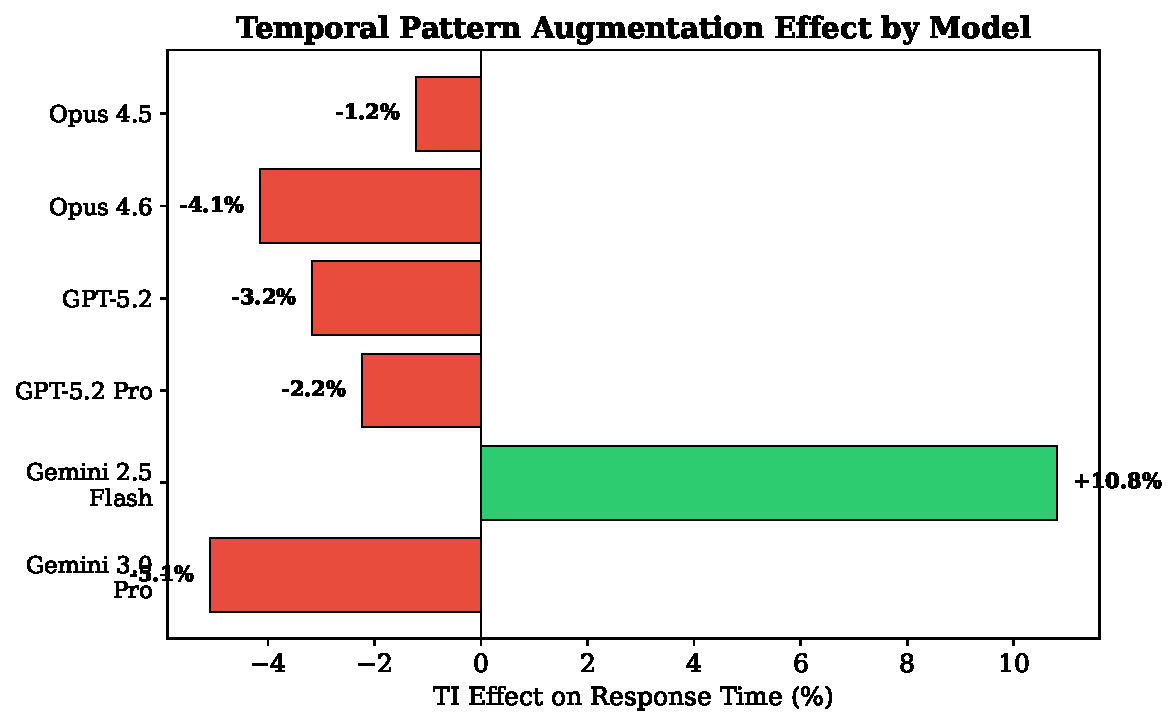
\includegraphics[width=0.85\textwidth]{figures/fig1_ti_effect_by_model.pdf}
\caption{TI effect (percentage change in response time) by model. Only Gemini 2.5 Flash shows a positive effect. All other models trend negative (slower with temporal augmentation).}
\label{fig:main_effect}
\end{figure}

\subsection{Capability--Effect Relationship}

Figure~\ref{fig:capability} plots each model's STATELESS pass rate against its TI effect, revealing a suggestive negative relationship: more capable models tend to be more negatively affected by temporal augmentation.

\begin{figure}[ht]
\centering
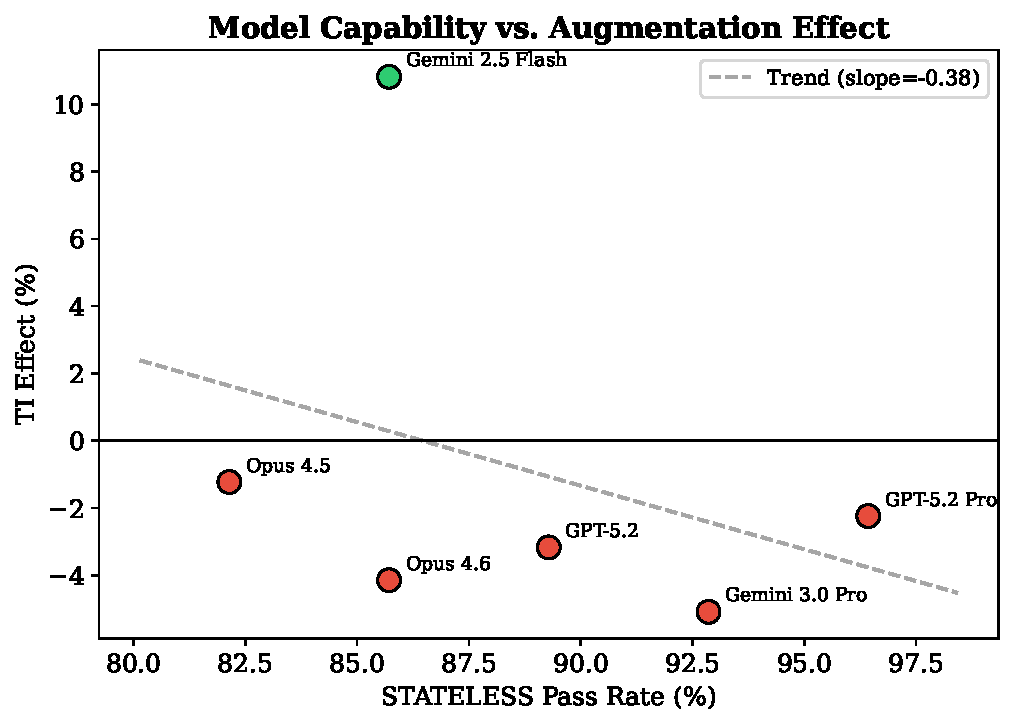
\includegraphics[width=0.7\textwidth]{figures/fig2_capability_vs_effect.pdf}
\caption{Model capability (STATELESS pass rate) vs.\ TI effect. Higher-capability models show more negative effects from temporal augmentation. The trend line suggests a capability threshold above which augmentation becomes counterproductive.}
\label{fig:capability}
\end{figure}

\subsection{Results by Difficulty}

Figure~\ref{fig:difficulty} breaks down response times by task difficulty. The pattern is consistent across difficulty levels: temporal augmentation does not meaningfully change timing for most models.

\begin{figure}[ht]
\centering
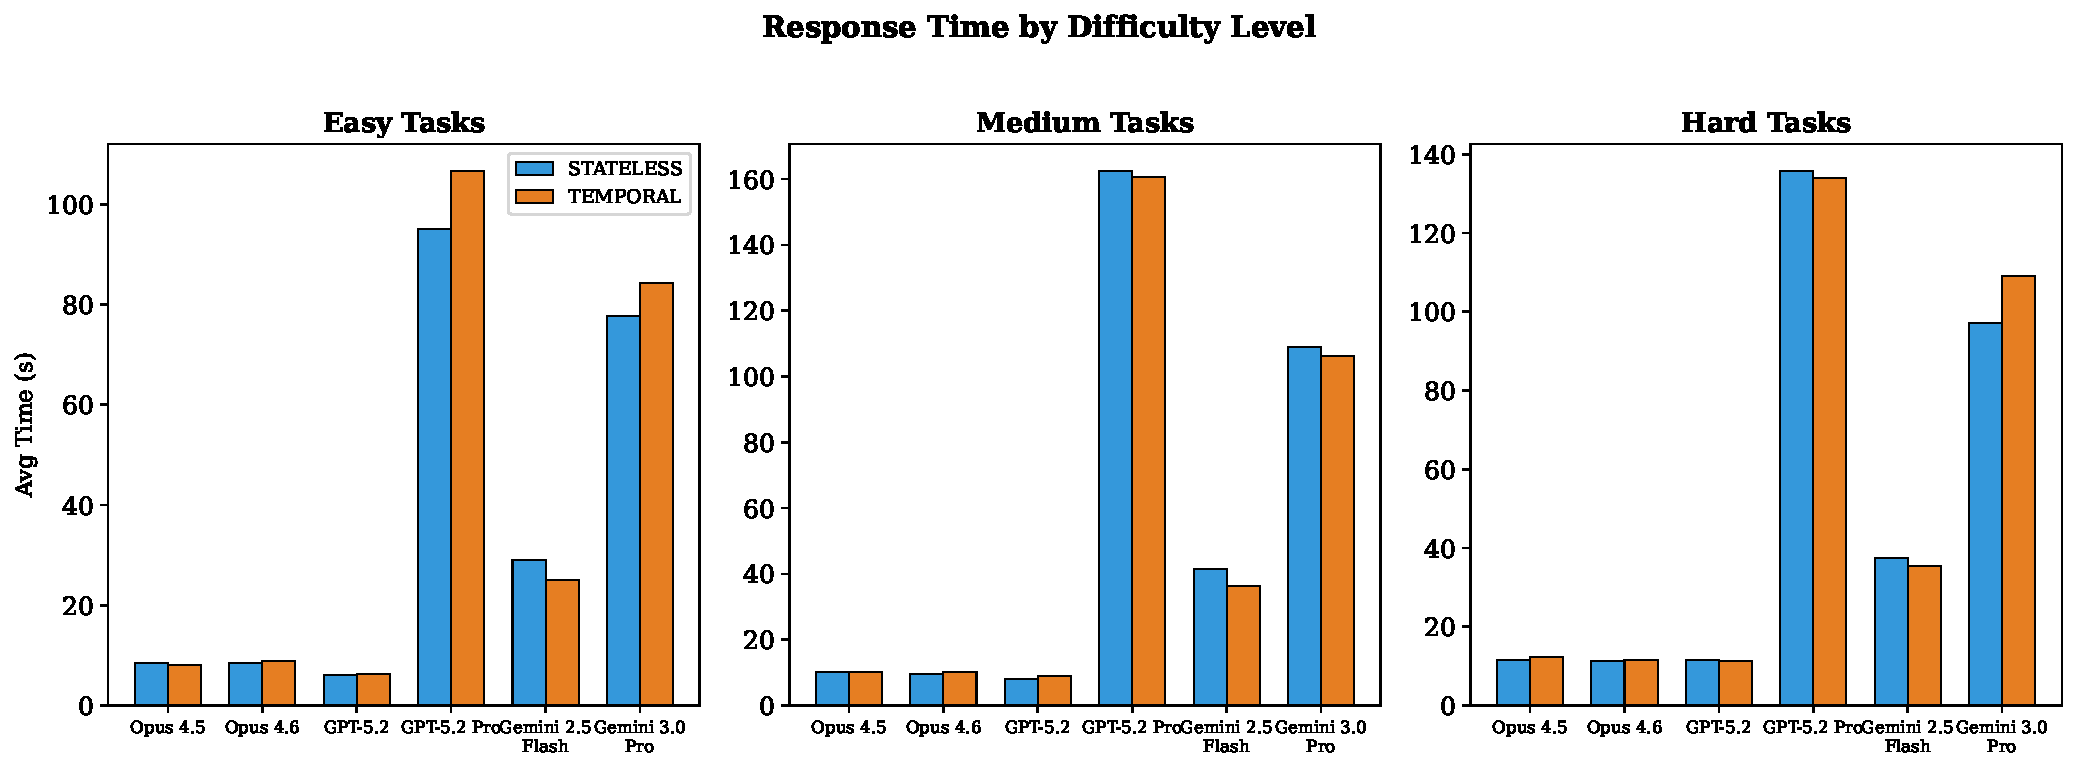
\includegraphics[width=\textwidth]{figures/fig3_timing_by_difficulty.pdf}
\caption{Average response time by difficulty level. STATELESS (blue) vs.\ TEMPORAL (orange) conditions for all six models. Differences are small and inconsistent across difficulty levels.}
\label{fig:difficulty}
\end{figure}

\subsection{Effect Sizes by Difficulty}

Figure~\ref{fig:heatmap} shows Cohen's $d$ for each model--difficulty combination. Effect sizes are uniformly small ($|d| < 0.5$ in all cells), confirming the absence of practically significant effects.

\begin{figure}[ht]
\centering
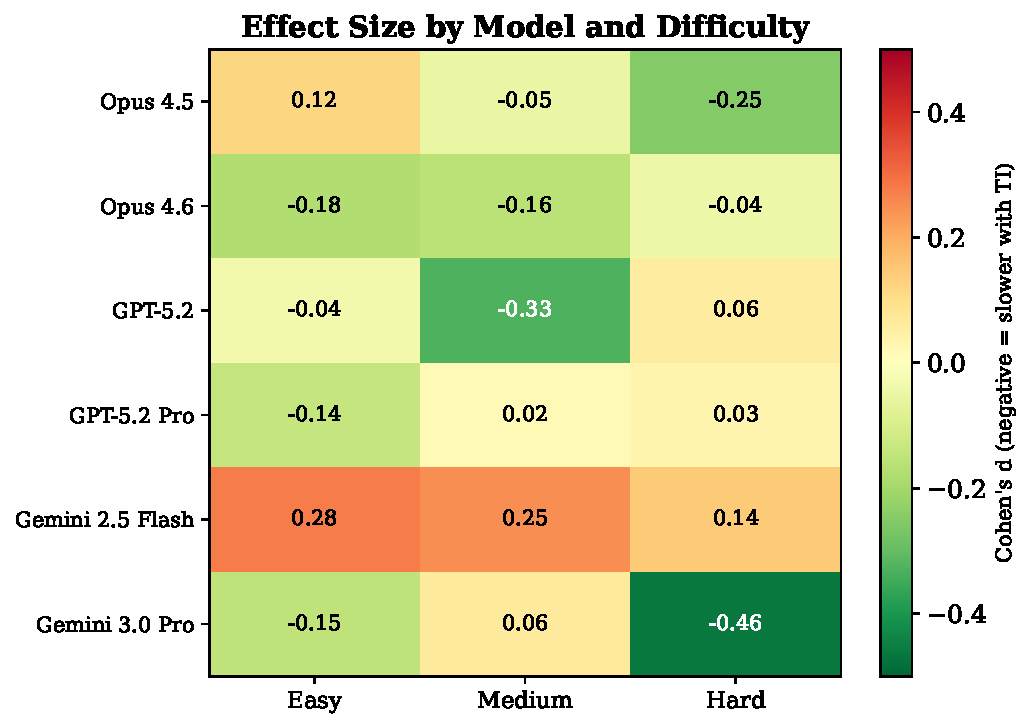
\includegraphics[width=0.7\textwidth]{figures/fig5_effect_size_heatmap.pdf}
\caption{Cohen's $d$ heatmap: models (rows) $\times$ difficulty (columns). Values near zero (yellow) indicate no effect. No cell exceeds the conventional ``medium'' threshold ($|d| = 0.5$).}
\label{fig:heatmap}
\end{figure}

%% ═══════════════════════════════════════════════════════════════
\section{The Capability Threshold Hypothesis}
\label{sec:threshold}

Our results suggest a \emph{capability threshold} for pattern augmentation: models below a certain capability level may benefit from external patterns, while models above it have already internalized those patterns.

\paragraph{Why Flash Benefits.} Gemini 2.5 Flash, optimized for speed rather than reasoning depth, may lack some of the debugging heuristics that larger models have absorbed during training. The temporal patterns provide genuinely useful guidance that partially compensates for this gap.

\paragraph{Why Stronger Models Degrade.} For Opus 4.5/4.6, GPT-5.2/5.2 Pro, and Gemini 3.0 Pro, the temporal context likely introduces \emph{processing overhead} without corresponding benefit. The model must parse and integrate 800--1200 additional tokens that largely duplicate its existing knowledge. This is consistent with findings in the RAG literature that irrelevant or redundant retrieval can hurt performance \citep{shi2023large}.

\paragraph{Implications.} The capability threshold is not fixed---it depends on the domain and the quality of the augmentation patterns. For highly specialized domains where training data is sparse, augmentation may help even strong models. For well-represented domains like code debugging, the threshold is already below current frontier models.

%% ═══════════════════════════════════════════════════════════════
\section{Measurement Artifact Analysis}
\label{sec:artifact}

Our earlier experiments, conducted through an orchestration layer (OpenClaw agent sessions), measured a \textbf{47\% speedup} for Opus 4.5 with temporal augmentation. This dramatic result motivated the cross-model study reported here. When we switched to direct API measurement, the effect for Opus 4.5 dropped to \textbf{$-1.2\%$} (Figure~\ref{fig:artifact}).

\begin{figure}[ht]
\centering
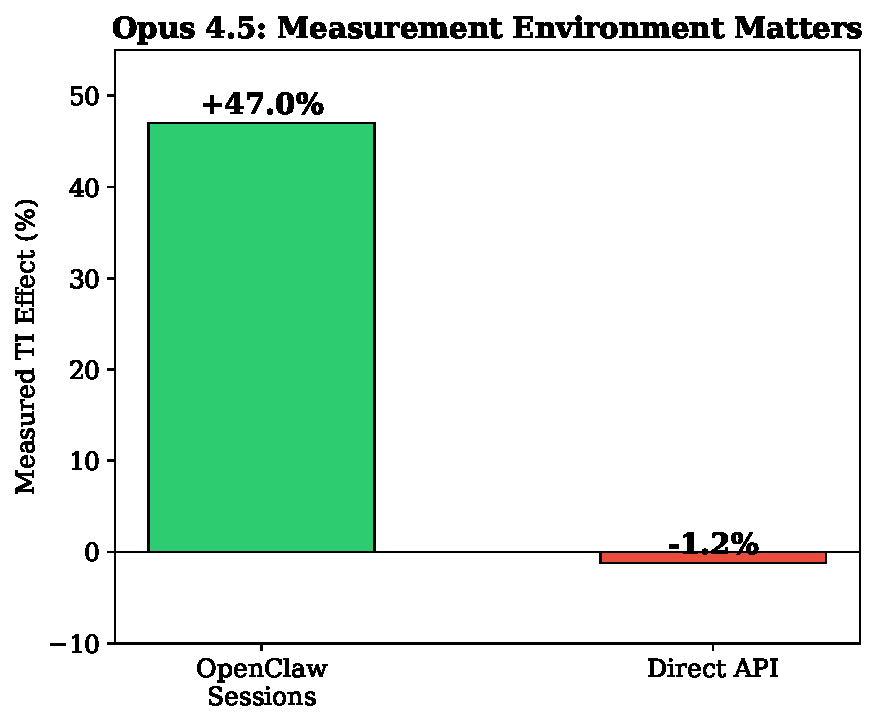
\includegraphics[width=0.55\textwidth]{figures/fig4_measurement_artifact.pdf}
\caption{The measurement artifact: identical model (Opus 4.5) and task suite measured through an orchestration layer (+47\%) vs.\ direct API ($-1.2\%$). The 48-point discrepancy is entirely attributable to the measurement environment.}
\label{fig:artifact}
\end{figure}

\paragraph{Root Cause.} The orchestration layer introduces variable overhead including session initialization, context management, tool routing, and response parsing. In the \textsc{Stateless} condition, the orchestration layer performed additional setup work (environment initialization without cached context), inflating baseline times. The \textsc{Temporal} condition benefited from pre-populated session state, creating an apparent speedup that was actually faster \emph{orchestration}, not faster \emph{model inference}.

\paragraph{Warning to the Community.} This artifact has broad implications for LLM benchmarking:
\begin{enumerate}[nosep]
    \item \textbf{Measure at the API level} whenever possible to isolate model behavior from infrastructure.
    \item \textbf{Be skeptical of large effects} measured through orchestration layers, agent frameworks, or multi-step pipelines.
    \item \textbf{Report measurement methodology} in detail, including whether timing includes infrastructure overhead.
\end{enumerate}

%% ═══════════════════════════════════════════════════════════════
\section{Discussion}
\label{sec:discussion}

\paragraph{When Does Augmentation Help?} Our results suggest that pattern augmentation helps when there is a genuine capability gap---when the model lacks knowledge that the patterns provide. For Gemini 2.5 Flash, the debugging heuristics in our temporal patterns appear to partially fill such a gap. For stronger models, no gap exists for this task domain.

\paragraph{Cost Implications.} Temporal augmentation adds 800--1200 tokens per request. At current API pricing, this represents a non-trivial cost increase (5--15\% depending on model and task length) for zero or negative benefit on capable models. Practitioners should evaluate augmentation strategies against their specific model and domain rather than assuming universal benefit.

\paragraph{The ``More Context'' Assumption.} Our findings challenge the implicit assumption that more context is always better. While this assumption holds for knowledge the model lacks, it fails for knowledge the model already possesses. As models improve, the set of ``knowledge the model lacks'' shrinks, reducing the marginal value of augmentation.

\paragraph{Comparison to RAG.} Our findings parallel observations in the RAG literature: retrieval helps when it provides genuinely new information but can hurt when retrieved content is redundant or distracting \citep{shi2023large}. Temporal pattern augmentation, by providing patterns the model already knows, falls into the ``redundant'' category for strong models.

%% ═══════════════════════════════════════════════════════════════
\section{Limitations}
\label{sec:limitations}

\begin{enumerate}[nosep]
    \item \textbf{Single task domain.} All 28 tasks are code debugging. Results may not transfer to other domains (e.g., creative writing, mathematical reasoning, medical diagnosis).
    \item \textbf{Limited task count.} With 28 tasks, statistical power is limited. True small effects ($|d| < 0.2$) may not be detectable.
    \item \textbf{Human-curated patterns.} Our temporal patterns were manually created. Automatically extracted patterns might perform differently.
    \item \textbf{Single run per condition.} Each task was run once per condition per model. Run-to-run variance (especially for stochastic models at temperature 0 with variable server load) is not captured.
    \item \textbf{Fixed pattern design.} We used the same temporal context structure for all models. Model-specific pattern formats might yield different results.
    \item \textbf{Snapshot in time.} These results reflect model capabilities as of February 2026. Future model versions may respond differently to augmentation.
    \item \textbf{Response time as proxy.} We measure wall-clock API response time, which conflates thinking time with generation time and is subject to server-side variability.
\end{enumerate}

%% ═══════════════════════════════════════════════════════════════
\section{Conclusion}
\label{sec:conclusion}

We evaluated temporal pattern augmentation---injecting historical problem-solving patterns into LLM prompts---across six foundation models on 28 code debugging tasks. Our central finding is negative: \textbf{temporal augmentation does not improve performance for five of six models tested}, with only the least capable model (Gemini 2.5 Flash) showing a modest, non-significant speedup of +10.8\%.

This negative result carries three positive contributions:
\begin{enumerate}[nosep]
    \item \textbf{A capability threshold for augmentation}: As models improve, the marginal value of pattern injection decreases, eventually becoming counterproductive.
    \item \textbf{A measurement artifact warning}: A previously reported 47\% speedup was entirely attributable to orchestration-layer overhead, not model behavior. This cautionary finding applies broadly to LLM benchmarking.
    \item \textbf{Practical guidance}: For current frontier models on well-represented task domains, practitioners should not invest in historical pattern augmentation systems. Resources are better spent on task-specific prompt engineering or domain expansion.
\end{enumerate}

The experimental design (Figure~\ref{fig:design}) and all data are available at \url{https://github.com/engagedirect001/temporalintelligence}.

\begin{figure}[ht]
\centering
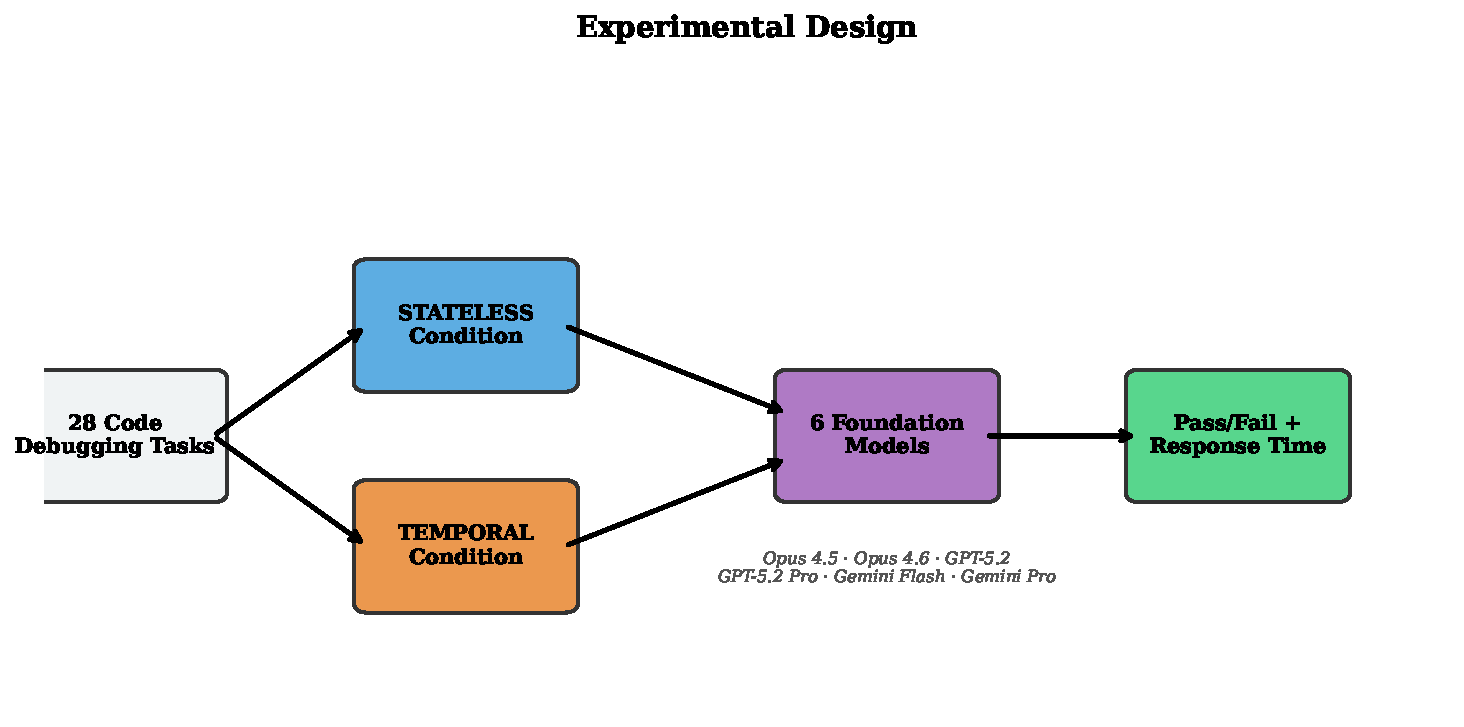
\includegraphics[width=0.85\textwidth]{figures/fig6_experimental_design.pdf}
\caption{Experimental design overview. 28 debugging tasks are presented in two conditions (STATELESS and TEMPORAL) to six foundation models, measuring pass/fail and response time.}
\label{fig:design}
\end{figure}

\bibliographystyle{plainnat}

\begin{thebibliography}{10}

\bibitem[Brown et~al.(2020)]{brown2020language}
T.~Brown, B.~Mann, N.~Ryder, et~al.
\newblock Language models are few-shot learners.
\newblock In \emph{NeurIPS}, 2020.

\bibitem[Finn et~al.(2017)]{finn2017model}
C.~Finn, P.~Abbeel, and S.~Levine.
\newblock Model-agnostic meta-learning for fast adaptation of deep networks.
\newblock In \emph{ICML}, 2017.

\bibitem[Lewis et~al.(2020)]{lewis2020retrieval}
P.~Lewis, E.~Perez, A.~Piktus, et~al.
\newblock Retrieval-augmented generation for knowledge-intensive {NLP} tasks.
\newblock In \emph{NeurIPS}, 2020.

\bibitem[Min et~al.(2022)]{min2022rethinking}
S.~Min, X.~Lyu, A.~Holtzman, et~al.
\newblock Rethinking the role of demonstrations: What makes in-context learning work?
\newblock In \emph{EMNLP}, 2022.

\bibitem[Packer et~al.(2023)]{packer2023memgpt}
C.~Packer, S.~Wooders, K.~Lin, et~al.
\newblock {MemGPT}: Towards {LLMs} as operating systems.
\newblock \emph{arXiv preprint arXiv:2310.08560}, 2023.

\bibitem[Rogers et~al.(2020)]{rogers2020primer}
A.~Rogers, O.~Kovaleva, and A.~Rumshisky.
\newblock A primer in {BERTology}: What we know about how {BERT} works.
\newblock \emph{TACL}, 8:842--866, 2020.

\bibitem[Shi et~al.(2023)]{shi2023large}
F.~Shi, X.~Chen, K.~Misra, et~al.
\newblock Large language models can be easily distracted by irrelevant context.
\newblock In \emph{ICML}, 2023.

\bibitem[Shinn et~al.(2023)]{shinn2023reflexion}
N.~Shinn, F.~Cassano, E.~Berman, et~al.
\newblock Reflexion: Language agents with verbal reinforcement learning.
\newblock In \emph{NeurIPS}, 2023.

\bibitem[Wei et~al.(2022)]{wei2022chain}
J.~Wei, X.~Wang, D.~Schuurmans, et~al.
\newblock Chain-of-thought prompting elicits reasoning in large language models.
\newblock In \emph{NeurIPS}, 2022.

\end{thebibliography}

\end{document}
